% ========================================
% PARTE 2: EJEMPLOS RESUELTOS Y EJERCICIOS INVERSOS
% Gráficas de Funciones Trigonométricas
% ========================================

\section{Ejemplos Resueltos}

Ahora vamos a ver cómo graficar las seis funciones trigonométricas. Cada ejemplo incluye una construcción detallada de la gráfica paso a paso, para que entiendas no solo cómo se ve, sino también por qué se ve así.

\begin{ejemplo}[title=Ejemplo 1: Graficar la funcion seno]
Grafica la función $y = \sin(x)$ en el intervalo $[0°, 360°]$ e identifica sus características principales.

\vspace{0.3cm}
\textbf{Solución:}

\textbf{Paso 1:} Construir una tabla de valores para ángulos especiales.

Vamos a usar los ángulos especiales que conocemos: $0°, 30°, 45°, 60°, 90°, 120°, 135°, 150°, 180°$, etc.

\begin{center}
\renewcommand{\arraystretch}{1.5}
\begin{tabular}{|c|c|c|c|c|c|c|c|c|c|}
\hline
$x$ & $0°$ & $30°$ & $60°$ & $90°$ & $120°$ & $150°$ & $180°$ & $210°$ & $240°$ \\
\hline
$\sin(x)$ & $0$ & $0.5$ & $0.87$ & $1$ & $0.87$ & $0.5$ & $0$ & $-0.5$ & $-0.87$ \\
\hline
\end{tabular}
\end{center}

\begin{center}
\renewcommand{\arraystretch}{1.5}
\begin{tabular}{|c|c|c|c|c|}
\hline
$x$ & $270°$ & $300°$ & $330°$ & $360°$ \\
\hline
$\sin(x)$ & $-1$ & $-0.87$ & $-0.5$ & $0$ \\
\hline
\end{tabular}
\end{center}

\textbf{Paso 2:} Analizar el comportamiento de la función.

\begin{itemize}
    \item La función \textbf{comienza en 0} cuando $x = 0°$
    \item \textbf{Crece} hasta alcanzar el máximo valor de 1 en $x = 90°$
    \item \textbf{Decrece} volviendo a 0 en $x = 180°$
    \item \textbf{Continúa decreciendo} hasta el mínimo valor de $-1$ en $x = 270°$
    \item \textbf{Regresa a 0} cuando $x = 360°$
\end{itemize}

\textbf{Paso 3:} Trazar la gráfica.

\begin{center}
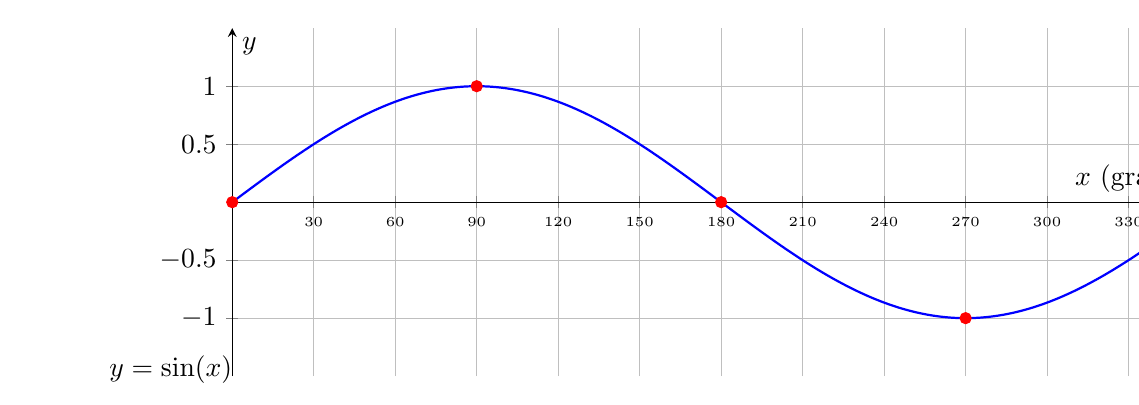
\begin{tikzpicture}
\begin{axis}[
    width=14cm,
    height=6cm,
    axis lines=center,
    xlabel={$x$ (grados)},
    ylabel={$y$},
    xmin=0, xmax=360,
    ymin=-1.5, ymax=1.5,
    xtick={0,30,60,90,120,150,180,210,240,270,300,330,360},
    xticklabels={$0°$,$30°$,$60°$,$90°$,$120°$,$150°$,$180°$,$210°$,$240°$,$270°$,$300°$,$330°$,$360°$},
    xticklabel style={font=\tiny},
    ytick={-1,-0.5,0,0.5,1},
    grid=both,
    grid style={line width=.1pt, draw=gray!10},
    major grid style={line width=.2pt,draw=gray!50},
    legend pos=north east,
]
    % Gráfica de seno
    \addplot[
        domain=0:360,
        samples=200,
        smooth,
        thick,
        color=blue,
    ] {sin(x)};
    \addlegend{$y = \sin(x)$}

    % Puntos importantes
    \addplot[only marks, mark=*, mark size=2pt, color=red] coordinates {
        (0,0) (90,1) (180,0) (270,-1) (360,0)
    };
\end{axis}
\end{tikzpicture}
\end{center}

\textbf{Paso 4:} Identificar las características.

\begin{itemize}
    \item \textbf{Dominio:} Todos los números reales (en este caso, todos los ángulos)
    \item \textbf{Rango:} $[-1, 1]$
    \item \textbf{Período:} $360°$ (la función se repite cada $360°$)
    \item \textbf{Amplitud:} 1 (distancia del centro a un máximo o mínimo)
    \item \textbf{Máximos:} En $x = 90°, 450°, 810°,\ldots$ (cada $90° + 360°k$)
    \item \textbf{Mínimos:} En $x = 270°, 630°, 990°,\ldots$ (cada $270° + 360°k$)
    \item \textbf{Ceros:} En $x = 0°, 180°, 360°, 540°,\ldots$ (cada $180°k$)
    \item \textbf{Simetría:} Impar (simétrica respecto al origen)
\end{itemize}

\textbf{Respuesta:} La gráfica muestra el comportamiento ondulatorio característico de la función seno, con oscilaciones suaves entre $-1$ y $1$.
\end{ejemplo}

\begin{ejemplo}[title=Ejemplo 2: Graficar la funcion coseno]
Grafica la función $y = \cos(x)$ en el intervalo $[0°, 360°]$ y compárala con la función seno.

\vspace{0.3cm}
\textbf{Solución:}

\textbf{Paso 1:} Construir tabla de valores.

\begin{center}
\renewcommand{\arraystretch}{1.5}
\begin{tabular}{|c|c|c|c|c|c|c|c|c|c|}
\hline
$x$ & $0°$ & $30°$ & $60°$ & $90°$ & $120°$ & $150°$ & $180°$ & $210°$ & $240°$ \\
\hline
$\cos(x)$ & $1$ & $0.87$ & $0.5$ & $0$ & $-0.5$ & $-0.87$ & $-1$ & $-0.87$ & $-0.5$ \\
\hline
\end{tabular}
\end{center}

\begin{center}
\renewcommand{\arraystretch}{1.5}
\begin{tabular}{|c|c|c|c|c|}
\hline
$x$ & $270°$ & $300°$ & $330°$ & $360°$ \\
\hline
$\cos(x)$ & $0$ & $0.5$ & $0.87$ & $1$ \\
\hline
\end{tabular}
\end{center}

\textbf{Paso 2:} Analizar el comportamiento.

\begin{itemize}
    \item La función \textbf{comienza en su máximo} valor de 1 cuando $x = 0°$
    \item \textbf{Decrece} hasta llegar a 0 en $x = 90°$
    \item \textbf{Continúa decreciendo} hasta el mínimo de $-1$ en $x = 180°$
    \item \textbf{Crece} nuevamente hasta 0 en $x = 270°$
    \item \textbf{Regresa al máximo} de 1 cuando $x = 360°$
\end{itemize}

\textbf{Paso 3:} Trazar la gráfica.

\begin{center}
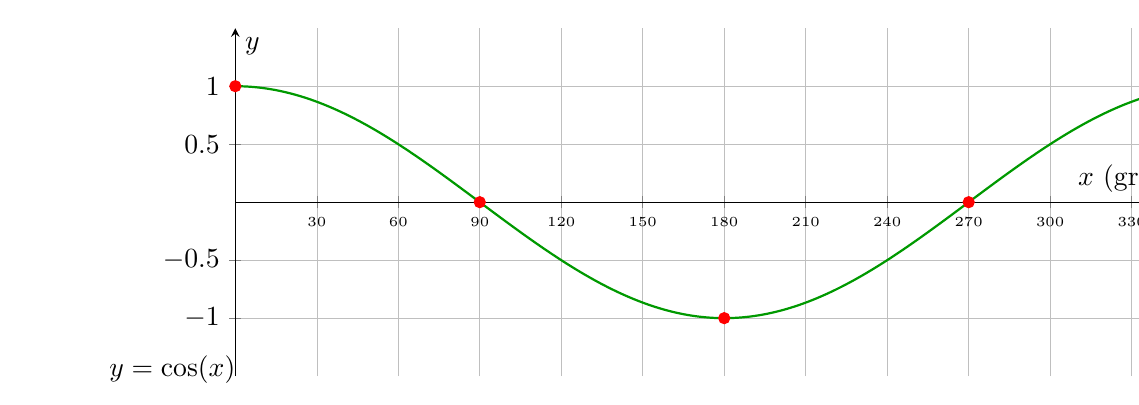
\begin{tikzpicture}
\begin{axis}[
    width=14cm,
    height=6cm,
    axis lines=center,
    xlabel={$x$ (grados)},
    ylabel={$y$},
    xmin=0, xmax=360,
    ymin=-1.5, ymax=1.5,
    xtick={0,30,60,90,120,150,180,210,240,270,300,330,360},
    xticklabels={$0°$,$30°$,$60°$,$90°$,$120°$,$150°$,$180°$,$210°$,$240°$,$270°$,$300°$,$330°$,$360°$},
    xticklabel style={font=\tiny},
    ytick={-1,-0.5,0,0.5,1},
    grid=both,
    grid style={line width=.1pt, draw=gray!10},
    major grid style={line width=.2pt,draw=gray!50},
    legend pos=north east,
]
    % Gráfica de coseno
    \addplot[
        domain=0:360,
        samples=200,
        smooth,
        thick,
        color=green!60!black,
    ] {cos(x)};
    \addlegend{$y = \cos(x)$}

    % Puntos importantes
    \addplot[only marks, mark=*, mark size=2pt, color=red] coordinates {
        (0,1) (90,0) (180,-1) (270,0) (360,1)
    };
\end{axis}
\end{tikzpicture}
\end{center}

\textbf{Paso 4:} Identificar características.

\begin{itemize}
    \item \textbf{Dominio:} Todos los números reales
    \item \textbf{Rango:} $[-1, 1]$
    \item \textbf{Período:} $360°$
    \item \textbf{Amplitud:} 1
    \item \textbf{Máximos:} En $x = 0°, 360°, 720°,\ldots$ (cada $360°k$)
    \item \textbf{Mínimos:} En $x = 180°, 540°, 900°,\ldots$ (cada $180° + 360°k$)
    \item \textbf{Ceros:} En $x = 90°, 270°, 450°,\ldots$ (cada $90° + 180°k$)
    \item \textbf{Simetría:} Par (simétrica respecto al eje y)
\end{itemize}

\textbf{Paso 5:} Comparación con la función seno.

\begin{center}
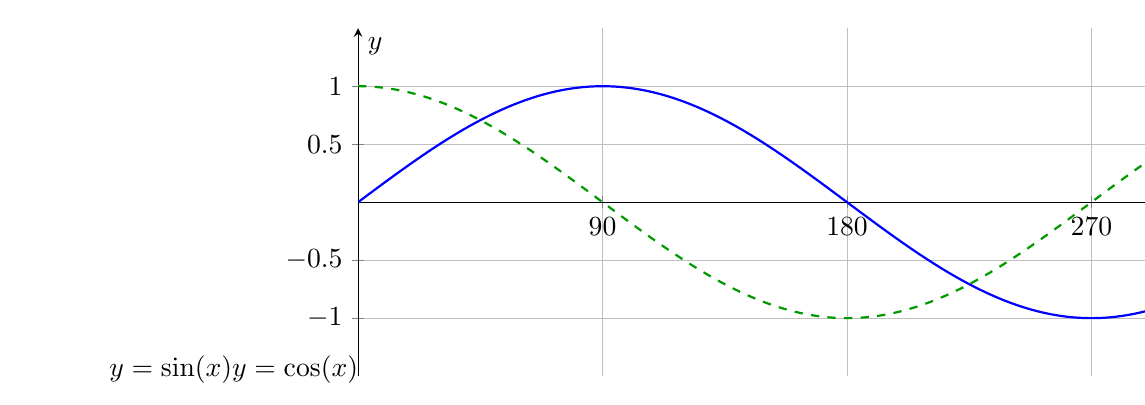
\begin{tikzpicture}
\begin{axis}[
    width=14cm,
    height=6cm,
    axis lines=center,
    xlabel={$x$ (grados)},
    ylabel={$y$},
    xmin=0, xmax=360,
    ymin=-1.5, ymax=1.5,
    xtick={0,90,180,270,360},
    xticklabels={$0°$,$90°$,$180°$,$270°$,$360°$},
    ytick={-1,-0.5,0,0.5,1},
    grid=both,
    grid style={line width=.1pt, draw=gray!10},
    major grid style={line width=.2pt,draw=gray!50},
    legend pos=north east,
]
    % Seno
    \addplot[
        domain=0:360,
        samples=200,
        smooth,
        thick,
        color=blue,
    ] {sin(x)};

    % Coseno
    \addplot[
        domain=0:360,
        samples=200,
        smooth,
        thick,
        color=green!60!black,
        dashed,
    ] {cos(x)};

    \addlegend{$y = \sin(x)$, $y = \cos(x)$}
\end{axis}
\end{tikzpicture}
\end{center}

\textbf{Observación clave:} La gráfica del coseno es idéntica a la del seno, pero \textbf{desplazada $90°$ hacia la izquierda}. De hecho, se cumple que: $\cos(x) = \sin(x + 90°)$

\textbf{Respuesta:} La función coseno tiene la misma forma ondulante que la función seno, pero comienza en su valor máximo.
\end{ejemplo}

\begin{ejemplo}[title=Ejemplo 3: Graficar la funcion tangente]
Grafica la función $y = \tan(x)$ en el intervalo $[0°, 360°]$ e identifica las asíntotas verticales.

\vspace{0.3cm}
\textbf{Solución:}

\textbf{Paso 1:} Recordar la definición.

La tangente se define como:
\[
\tan(x) = \frac{\sin(x)}{\cos(x)}
\]

Esto significa que la tangente \textbf{no está definida} cuando $\cos(x) = 0$, es decir, en $x = 90°, 270°, 450°,\ldots$

\textbf{Paso 2:} Construir tabla de valores (evitando los puntos donde no está definida).

\begin{center}
\renewcommand{\arraystretch}{1.5}
\begin{tabular}{|c|c|c|c|c|c|c|c|}
\hline
$x$ & $0°$ & $30°$ & $45°$ & $60°$ & $120°$ & $135°$ & $150°$ \\
\hline
$\tan(x)$ & $0$ & $0.58$ & $1$ & $1.73$ & $-1.73$ & $-1$ & $-0.58$ \\
\hline
\end{tabular}
\end{center}

\begin{center}
\renewcommand{\arraystretch}{1.5}
\begin{tabular}{|c|c|c|c|c|c|c|}
\hline
$x$ & $180°$ & $210°$ & $225°$ & $240°$ & $300°$ & $360°$ \\
\hline
$\tan(x)$ & $0$ & $0.58$ & $1$ & $1.73$ & $-1.73$ & $0$ \\
\hline
\end{tabular}
\end{center}

\textbf{Paso 3:} Identificar las asíntotas verticales.

La función tiene asíntotas verticales (líneas que la función se acerca pero nunca toca) en:
\[
x = 90°, \quad x = 270°
\]

\textbf{Paso 4:} Trazar la gráfica.

\begin{center}
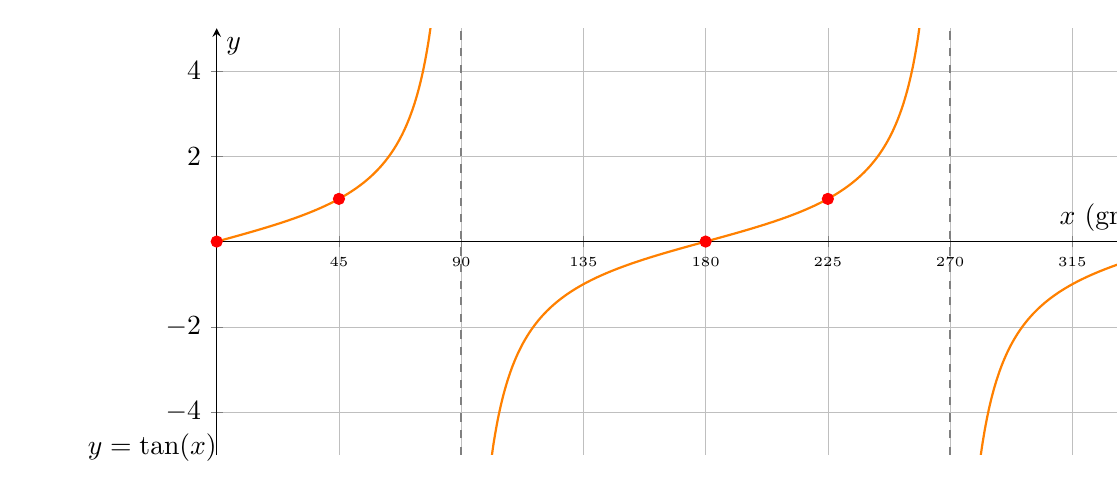
\begin{tikzpicture}
\begin{axis}[
    width=14cm,
    height=7cm,
    axis lines=center,
    xlabel={$x$ (grados)},
    ylabel={$y$},
    xmin=0, xmax=360,
    ymin=-5, ymax=5,
    xtick={0,45,90,135,180,225,270,315,360},
    xticklabels={$0°$,$45°$,$90°$,$135°$,$180°$,$225°$,$270°$,$315°$,$360°$},
    xticklabel style={font=\tiny},
    ytick={-4,-2,0,2,4},
    grid=both,
    grid style={line width=.1pt, draw=gray!10},
    major grid style={line width=.2pt,draw=gray!50},
    legend pos=north east,
    restrict y to domain=-6:6,
]
    % Asíntotas verticales
    \addplot[dashed, gray, thick, samples=2] coordinates {(90,-5) (90,5)};
    \addplot[dashed, gray, thick, samples=2] coordinates {(270,-5) (270,5)};

    % Gráfica de tangente
    \addplot[
        domain=0:89,
        samples=100,
        smooth,
        thick,
        color=orange,
    ] {tan(x)};

    \addplot[
        domain=91:269,
        samples=100,
        smooth,
        thick,
        color=orange,
    ] {tan(x)};

    \addplot[
        domain=271:360,
        samples=100,
        smooth,
        thick,
        color=orange,
    ] {tan(x)};

    \addlegend{$y = \tan(x)$}

    % Puntos importantes
    \addplot[only marks, mark=*, mark size=2pt, color=red] coordinates {
        (0,0) (45,1) (180,0) (225,1) (360,0)
    };
\end{axis}
\end{tikzpicture}
\end{center}

\textbf{Paso 5:} Identificar características.

\begin{itemize}
    \item \textbf{Dominio:} Todos los reales excepto $x = 90° + 180°k$ (donde $k$ es un entero)
    \item \textbf{Rango:} Todos los números reales $(-\infty, \infty)$
    \item \textbf{Período:} $180°$ (¡la mitad que seno y coseno!)
    \item \textbf{Asíntotas verticales:} En $x = 90°, 270°, 450°,\ldots$
    \item \textbf{Ceros:} En $x = 0°, 180°, 360°,\ldots$ (cada $180°k$)
    \item \textbf{Simetría:} Impar (simétrica respecto al origen)
    \item \textbf{Comportamiento:} Crece sin límite al acercarse a las asíntotas
\end{itemize}

\textbf{Verificación:} Comprobemos algunos valores:
\begin{align*}
\tan(0°) &= \frac{\sin(0°)}{\cos(0°)} = \frac{0}{1} = 0 \quad \checkmark \\
\tan(45°) &= \frac{\sin(45°)}{\cos(45°)} = \frac{\sqrt{2}/2}{\sqrt{2}/2} = 1 \quad \checkmark \\
\tan(90°) &= \frac{\sin(90°)}{\cos(90°)} = \frac{1}{0} = \text{indefinido} \quad \checkmark
\end{align*}

\textbf{Respuesta:} La función tangente tiene un comportamiento periódico con asíntotas verticales y crece indefinidamente entre ellas.
\end{ejemplo}

\begin{ejemplo}[title=Ejemplo 4: Graficar la funcion cotangente]
Grafica la función $y = \cot(x)$ en el intervalo $[0°, 360°]$ y compárala con la tangente.

\vspace{0.3cm}
\textbf{Solución:}

\textbf{Paso 1:} Recordar la definición.

La cotangente es la recíproca de la tangente:
\[
\cot(x) = \frac{1}{\tan(x)} = \frac{\cos(x)}{\sin(x)}
\]

Por lo tanto, \textbf{no está definida} cuando $\sin(x) = 0$, es decir, en $x = 0°, 180°, 360°,\ldots$

\textbf{Paso 2:} Construir tabla de valores.

\begin{center}
\renewcommand{\arraystretch}{1.5}
\begin{tabular}{|c|c|c|c|c|c|c|c|}
\hline
$x$ & $30°$ & $45°$ & $60°$ & $90°$ & $120°$ & $135°$ & $150°$ \\
\hline
$\cot(x)$ & $1.73$ & $1$ & $0.58$ & $0$ & $-0.58$ & $-1$ & $-1.73$ \\
\hline
\end{tabular}
\end{center}

\begin{center}
\renewcommand{\arraystretch}{1.5}
\begin{tabular}{|c|c|c|c|c|c|}
\hline
$x$ & $210°$ & $225°$ & $240°$ & $270°$ & $300°$ \\
\hline
$\cot(x)$ & $1.73$ & $1$ & $0.58$ & $0$ & $-0.58$ \\
\hline
\end{tabular}
\end{center}

\textbf{Paso 3:} Identificar las asíntotas verticales.

Las asíntotas verticales están en:
\[
x = 0°, \quad x = 180°, \quad x = 360°
\]

\textbf{Paso 4:} Trazar la gráfica.

\begin{center}
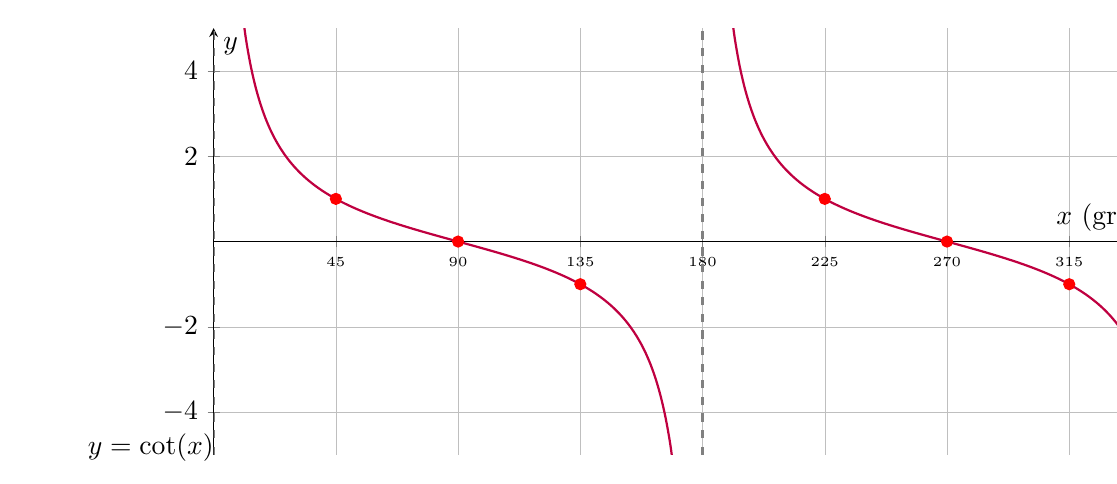
\begin{tikzpicture}
\begin{axis}[
    width=14cm,
    height=7cm,
    axis lines=center,
    xlabel={$x$ (grados)},
    ylabel={$y$},
    xmin=0, xmax=360,
    ymin=-5, ymax=5,
    xtick={0,45,90,135,180,225,270,315,360},
    xticklabels={$0°$,$45°$,$90°$,$135°$,$180°$,$225°$,$270°$,$315°$,$360°$},
    xticklabel style={font=\tiny},
    ytick={-4,-2,0,2,4},
    grid=both,
    grid style={line width=.1pt, draw=gray!10},
    major grid style={line width=.2pt,draw=gray!50},
    legend pos=north east,
    restrict y to domain=-6:6,
]
    % Asíntotas verticales
    \addplot[dashed, gray, thick, samples=2] coordinates {(0,-5) (0,5)};
    \addplot[dashed, gray, thick, samples=2] coordinates {(180,-5) (180,5)};
    \addplot[dashed, gray, thick, samples=2] coordinates {(360,-5) (360,5)};

    % Gráfica de cotangente
    \addplot[
        domain=1:179,
        samples=100,
        smooth,
        thick,
        color=purple,
    ] {cot(x)};

    \addplot[
        domain=181:359,
        samples=100,
        smooth,
        thick,
        color=purple,
    ] {cot(x)};

    \addlegend{$y = \cot(x)$}

    % Puntos importantes
    \addplot[only marks, mark=*, mark size=2pt, color=red] coordinates {
        (45,1) (90,0) (135,-1) (225,1) (270,0) (315,-1)
    };
\end{axis}
\end{tikzpicture}
\end{center}

\textbf{Paso 5:} Identificar características.

\begin{itemize}
    \item \textbf{Dominio:} Todos los reales excepto $x = 180°k$ (donde $k$ es un entero)
    \item \textbf{Rango:} Todos los números reales $(-\infty, \infty)$
    \item \textbf{Período:} $180°$
    \item \textbf{Asíntotas verticales:} En $x = 0°, 180°, 360°,\ldots$
    \item \textbf{Ceros:} En $x = 90°, 270°, 450°,\ldots$ (cada $90° + 180°k$)
    \item \textbf{Simetría:} Impar (simétrica respecto al origen)
    \item \textbf{Comportamiento:} Decrece desde $+\infty$ hasta $-\infty$ en cada período
\end{itemize}

\textbf{Paso 6:} Comparación con la tangente.

\begin{nota}
Observa que la cotangente es como una "reflexión" de la tangente:
\begin{itemize}
    \item Donde la tangente es cero, la cotangente tiene asíntotas
    \item Donde la tangente tiene asíntotas, la cotangente es cero
    \item La tangente crece; la cotangente decrece
\end{itemize}
\end{nota}

\textbf{Respuesta:} La función cotangente decrece continuamente en cada intervalo entre asíntotas, comportándose como la función recíproca de la tangente.
\end{ejemplo}

\begin{ejemplo}[title=Ejemplo 5: Graficar la funcion secante]
Grafica la función $y = \sec(x)$ en el intervalo $[0°, 360°]$ junto con $y = \cos(x)$ para visualizar su relación.

\vspace{0.3cm}
\textbf{Solución:}

\textbf{Paso 1:} Recordar la definición.

La secante es la recíproca del coseno:
\[
\sec(x) = \frac{1}{\cos(x)}
\]

Por lo tanto, \textbf{no está definida} cuando $\cos(x) = 0$, es decir, en $x = 90°, 270°,\ldots$

\textbf{Paso 2:} Analizar el comportamiento.

\begin{itemize}
    \item Cuando $\cos(x) = 1$, entonces $\sec(x) = 1$
    \item Cuando $\cos(x) = -1$, entonces $\sec(x) = -1$
    \item Cuando $\cos(x) \to 0^+$, entonces $\sec(x) \to +\infty$
    \item Cuando $\cos(x) \to 0^-$, entonces $\sec(x) \to -\infty$
    \item Cuando $|\cos(x)| < 1$, entonces $|\sec(x)| > 1$
\end{itemize}

\textbf{Paso 3:} Construir tabla de valores.

\begin{center}
\renewcommand{\arraystretch}{1.5}
\begin{tabular}{|c|c|c|c|c|c|c|c|}
\hline
$x$ & $0°$ & $30°$ & $45°$ & $60°$ & $120°$ & $135°$ & $150°$ \\
\hline
$\sec(x)$ & $1$ & $1.15$ & $1.41$ & $2$ & $-2$ & $-1.41$ & $-1.15$ \\
\hline
\end{tabular}
\end{center}

\textbf{Paso 4:} Trazar la gráfica junto con el coseno.

\begin{center}
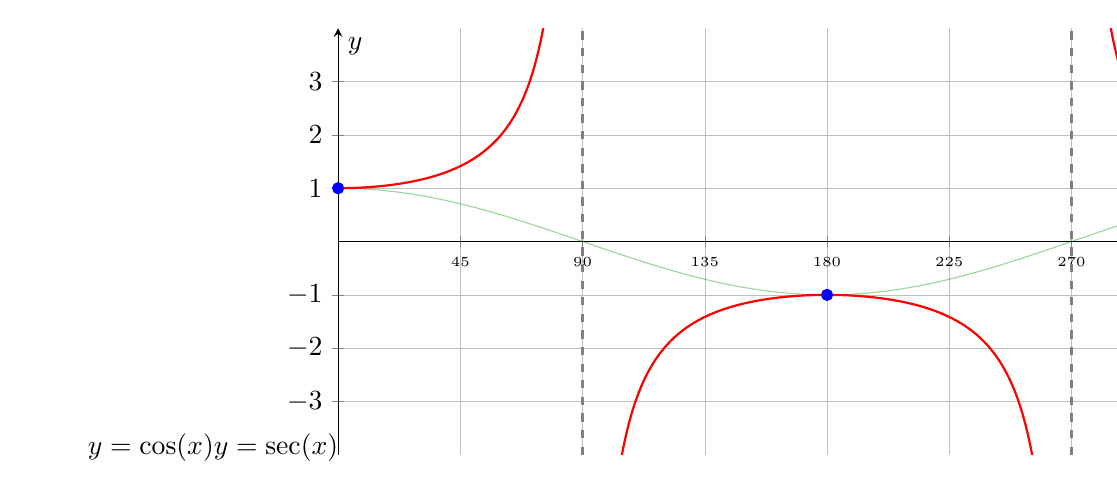
\begin{tikzpicture}
\begin{axis}[
    width=14cm,
    height=7cm,
    axis lines=center,
    xlabel={$x$ (grados)},
    ylabel={$y$},
    xmin=0, xmax=360,
    ymin=-4, ymax=4,
    xtick={0,45,90,135,180,225,270,315,360},
    xticklabels={$0°$,$45°$,$90°$,$135°$,$180°$,$225°$,$270°$,$315°$,$360°$},
    xticklabel style={font=\tiny},
    ytick={-3,-2,-1,0,1,2,3},
    grid=both,
    grid style={line width=.1pt, draw=gray!10},
    major grid style={line width=.2pt,draw=gray!50},
    legend pos=north east,
    restrict y to domain=-5:5,
]
    % Asíntotas verticales
    \addplot[dashed, gray, thick, samples=2] coordinates {(90,-4) (90,4)};
    \addplot[dashed, gray, thick, samples=2] coordinates {(270,-4) (270,4)};

    % Gráfica de coseno (para referencia)
    \addplot[
        domain=0:360,
        samples=200,
        smooth,
        thin,
        color=green!60!black,
        opacity=0.4,
    ] {cos(x)};

    % Gráfica de secante
    \addplot[
        domain=0:88,
        samples=100,
        smooth,
        thick,
        color=red,
    ] {1/cos(x)};

    \addplot[
        domain=92:268,
        samples=100,
        smooth,
        thick,
        color=red,
    ] {1/cos(x)};

    \addplot[
        domain=272:360,
        samples=100,
        smooth,
        thick,
        color=red,
    ] {1/cos(x)};

    \addlegend{$y = \cos(x)$, $y = \sec(x)$}

    % Puntos importantes
    \addplot[only marks, mark=*, mark size=2pt, color=blue] coordinates {
        (0,1) (180,-1) (360,1)
    };
\end{axis}
\end{tikzpicture}
\end{center}

\textbf{Paso 5:} Identificar características.

\begin{itemize}
    \item \textbf{Dominio:} Todos los reales excepto $x = 90° + 180°k$
    \item \textbf{Rango:} $(-\infty, -1] \cup [1, \infty)$ (¡nunca toma valores entre $-1$ y $1$!)
    \item \textbf{Período:} $360°$
    \item \textbf{Asíntotas verticales:} En $x = 90°, 270°, 450°,\ldots$
    \item \textbf{Valores extremos:} Mínimo de 1 en $x = 0°, 360°$; máximo de $-1$ en $x = 180°$
    \item \textbf{Simetría:} Par (simétrica respecto al eje y)
\end{itemize}

\textbf{Paso 6:} Relación con el coseno.

\begin{nota}
Observaciones importantes:
\begin{itemize}
    \item La gráfica de la secante \textbf{toca} la gráfica del coseno solo en los puntos donde $\cos(x) = \pm 1$
    \item Entre esos puntos, la secante forma "ramas" en forma de U (o U invertida)
    \item La secante está siempre \textbf{por encima} o \textbf{por debajo} del coseno, nunca entre $-1$ y $1$
\end{itemize}
\end{nota}

\textbf{Verificación:}
\begin{align*}
\sec(0°) &= \frac{1}{\cos(0°)} = \frac{1}{1} = 1 \quad \checkmark \\
\sec(60°) &= \frac{1}{\cos(60°)} = \frac{1}{1/2} = 2 \quad \checkmark \\
\sec(180°) &= \frac{1}{\cos(180°)} = \frac{1}{-1} = -1 \quad \checkmark
\end{align*}

\textbf{Respuesta:} La función secante forma ramas parabólicas que se alejan de la función coseno, con asíntotas donde el coseno se anula.
\end{ejemplo}

\begin{ejemplo}[title=Ejemplo 6: Graficar la funcion cosecante]
Grafica la función $y = \csc(x)$ en el intervalo $[0°, 360°]$ junto con $y = \sin(x)$ para entender su comportamiento.

\vspace{0.3cm}
\textbf{Solución:}

\textbf{Paso 1:} Recordar la definición.

La cosecante es la recíproca del seno:
\[
\csc(x) = \frac{1}{\sin(x)}
\]

Por lo tanto, \textbf{no está definida} cuando $\sin(x) = 0$, es decir, en $x = 0°, 180°, 360°,\ldots$

\textbf{Paso 2:} Analizar el comportamiento.

Similar a la secante con el coseno, la cosecante tiene una relación especial con el seno:

\begin{itemize}
    \item Cuando $\sin(x) = 1$, entonces $\csc(x) = 1$
    \item Cuando $\sin(x) = -1$, entonces $\csc(x) = -1$
    \item Cuando $\sin(x) \to 0^+$, entonces $\csc(x) \to +\infty$
    \item Cuando $\sin(x) \to 0^-$, entonces $\csc(x) \to -\infty$
    \item Cuando $|\sin(x)| < 1$, entonces $|\csc(x)| > 1$
\end{itemize}

\textbf{Paso 3:} Construir tabla de valores.

\begin{center}
\renewcommand{\arraystretch}{1.5}
\begin{tabular}{|c|c|c|c|c|c|c|c|}
\hline
$x$ & $30°$ & $45°$ & $60°$ & $90°$ & $120°$ & $135°$ & $150°$ \\
\hline
$\csc(x)$ & $2$ & $1.41$ & $1.15$ & $1$ & $1.15$ & $1.41$ & $2$ \\
\hline
\end{tabular}
\end{center}

\begin{center}
\renewcommand{\arraystretch}{1.5}
\begin{tabular}{|c|c|c|c|c|c|}
\hline
$x$ & $210°$ & $225°$ & $240°$ & $270°$ & $300°$ \\
\hline
$\csc(x)$ & $-2$ & $-1.41$ & $-1.15$ & $-1$ & $-1.15$ \\
\hline
\end{tabular}
\end{center}

\textbf{Paso 4:} Trazar la gráfica junto con el seno.

\begin{center}
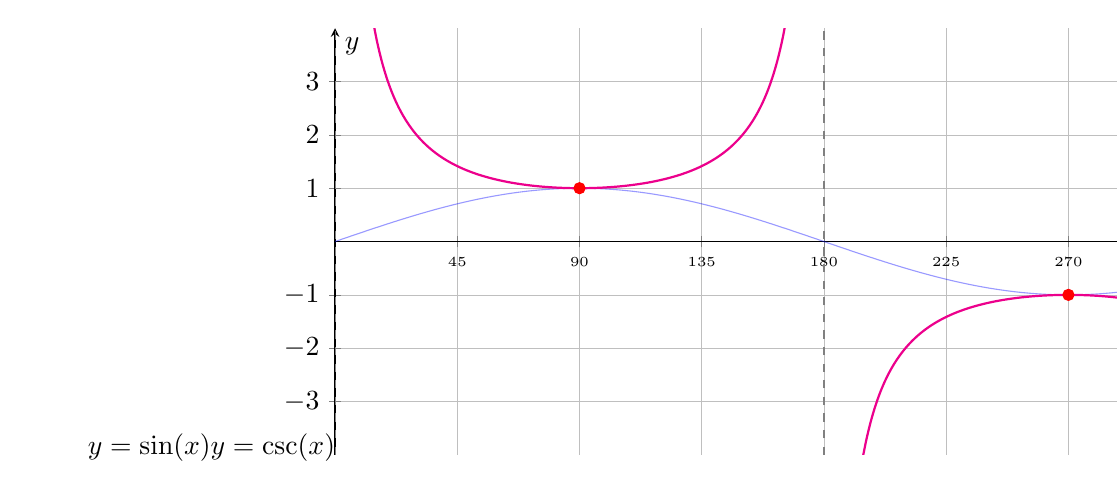
\begin{tikzpicture}
\begin{axis}[
    width=14cm,
    height=7cm,
    axis lines=center,
    xlabel={$x$ (grados)},
    ylabel={$y$},
    xmin=0, xmax=360,
    ymin=-4, ymax=4,
    xtick={0,45,90,135,180,225,270,315,360},
    xticklabels={$0°$,$45°$,$90°$,$135°$,$180°$,$225°$,$270°$,$315°$,$360°$},
    xticklabel style={font=\tiny},
    ytick={-3,-2,-1,0,1,2,3},
    grid=both,
    grid style={line width=.1pt, draw=gray!10},
    major grid style={line width=.2pt,draw=gray!50},
    legend pos=north east,
    restrict y to domain=-5:5,
]
    % Asíntotas verticales
    \addplot[dashed, gray, thick, samples=2] coordinates {(0,-4) (0,4)};
    \addplot[dashed, gray, thick, samples=2] coordinates {(180,-4) (180,4)};
    \addplot[dashed, gray, thick, samples=2] coordinates {(360,-4) (360,4)};

    % Gráfica de seno (para referencia)
    \addplot[
        domain=0:360,
        samples=200,
        smooth,
        thin,
        color=blue,
        opacity=0.4,
    ] {sin(x)};

    % Gráfica de cosecante
    \addplot[
        domain=1:179,
        samples=100,
        smooth,
        thick,
        color=magenta,
    ] {1/sin(x)};

    \addplot[
        domain=181:359,
        samples=100,
        smooth,
        thick,
        color=magenta,
    ] {1/sin(x)};

    \addlegend{$y = \sin(x)$, $y = \csc(x)$}

    % Puntos importantes
    \addplot[only marks, mark=*, mark size=2pt, color=red] coordinates {
        (90,1) (270,-1)
    };
\end{axis}
\end{tikzpicture}
\end{center}

\textbf{Paso 5:} Identificar características.

\begin{itemize}
    \item \textbf{Dominio:} Todos los reales excepto $x = 180°k$ (donde $k$ es un entero)
    \item \textbf{Rango:} $(-\infty, -1] \cup [1, \infty)$
    \item \textbf{Período:} $360°$
    \item \textbf{Asíntotas verticales:} En $x = 0°, 180°, 360°,\ldots$
    \item \textbf{Valores extremos:} Mínimo de 1 en $x = 90°$; máximo de $-1$ en $x = 270°$
    \item \textbf{Simetría:} Impar (simétrica respecto al origen)
\end{itemize}

\textbf{Paso 6:} Comparación con la secante.

\begin{center}
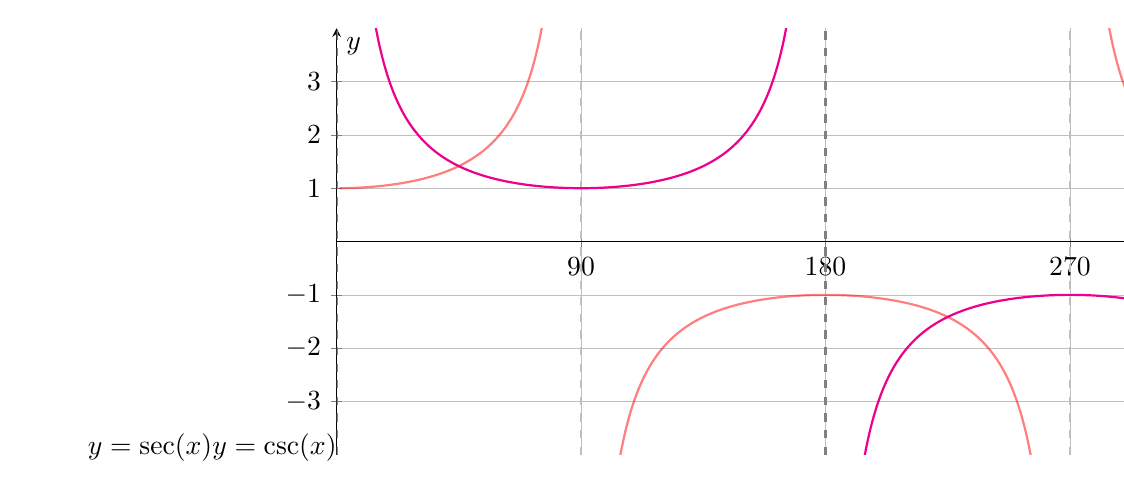
\begin{tikzpicture}
\begin{axis}[
    width=14cm,
    height=7cm,
    axis lines=center,
    xlabel={$x$ (grados)},
    ylabel={$y$},
    xmin=0, xmax=360,
    ymin=-4, ymax=4,
    xtick={0,90,180,270,360},
    ytick={-3,-2,-1,0,1,2,3},
    grid=both,
    grid style={line width=.1pt, draw=gray!10},
    major grid style={line width=.2pt,draw=gray!50},
    legend pos=north east,
    restrict y to domain=-5:5,
]
    % Asíntotas de secante
    \addplot[dashed, gray!50, samples=2] coordinates {(90,-4) (90,4)};
    \addplot[dashed, gray!50, samples=2] coordinates {(270,-4) (270,4)};

    % Asíntotas de cosecante
    \addplot[dashed, gray, thick, samples=2] coordinates {(0,-4) (0,4)};
    \addplot[dashed, gray, thick, samples=2] coordinates {(180,-4) (180,4)};
    \addplot[dashed, gray, thick, samples=2] coordinates {(360,-4) (360,4)};

    % Secante
    \addplot[
        domain=1:88,
        samples=100,
        smooth,
        thick,
        color=red,
        opacity=0.5,
    ] {1/cos(x)};

    \addplot[
        domain=92:268,
        samples=100,
        smooth,
        thick,
        color=red,
        opacity=0.5,
    ] {1/cos(x)};

    \addplot[
        domain=272:359,
        samples=100,
        smooth,
        thick,
        color=red,
        opacity=0.5,
    ] {1/cos(x)};

    % Cosecante
    \addplot[
        domain=1:179,
        samples=100,
        smooth,
        thick,
        color=magenta,
    ] {1/sin(x)};

    \addplot[
        domain=181:359,
        samples=100,
        smooth,
        thick,
        color=magenta,
    ] {1/sin(x)};

    \addlegend{$y = \sec(x)$, $y = \csc(x)$}
\end{axis}
\end{tikzpicture}
\end{center}

\textbf{Observación:} La cosecante está desplazada $90°$ respecto a la secante, de la misma manera que el seno está desplazado respecto al coseno.

\textbf{Verificación:}
\begin{align*}
\csc(30°) &= \frac{1}{\sin(30°)} = \frac{1}{1/2} = 2 \quad \checkmark \\
\csc(90°) &= \frac{1}{\sin(90°)} = \frac{1}{1} = 1 \quad \checkmark \\
\csc(270°) &= \frac{1}{\sin(270°)} = \frac{1}{-1} = -1 \quad \checkmark
\end{align*}

\textbf{Respuesta:} La función cosecante forma ramas parabólicas alternadas, con asíntotas verticales donde el seno se anula, comportándose como la función recíproca del seno.
\end{ejemplo}

\newpage

% ========================================
% EJERCICIOS INVERSOS
% ========================================

\section{Ejercicios Inversos}

Los ejercicios inversos te desafían a usar tu creatividad y comprensión profunda de las funciones trigonométricas. En lugar de simplemente graficar funciones dadas, deberás diseñar funciones que cumplan ciertas características.

\begin{ejercicio}[title=Ejercicio Inverso 1: Disenar una funcion con amplitud y periodo especificos]
Diseña una función trigonométrica basada en el seno que tenga las siguientes características:
\begin{itemize}
    \item Amplitud de 3
    \item Período de $180°$
    \item Que pase por el origen
\end{itemize}

Escribe la ecuación de la función y grafícala en el intervalo $[0°, 360°]$.
\end{ejercicio}

\begin{ejercicio}[title=Ejercicio Inverso 2: Identificar la funcion a partir de su grafica]
Se te proporciona la siguiente información sobre una función trigonométrica:
\begin{itemize}
    \item Tiene asíntotas verticales en $x = 0°, 180°, 360°$
    \item Es positiva en el intervalo $(0°, 90°)$
    \item Decrece en cada intervalo entre asíntotas
    \item Pasa por el punto $(45°, 1)$
\end{itemize}

Identifica qué función trigonométrica cumple estas características y justifica tu respuesta con una gráfica.
\end{ejercicio}

\begin{ejercicio}[title=Ejercicio Inverso 3: Crear una funcion compuesta]
Un ingeniero necesita modelar una señal que oscila entre $-2$ y $2$, con un período de $120°$, y que comienza en su valor máximo cuando $x = 0°$.

\begin{itemize}
    \item[a)] Determina qué función trigonométrica (seno o coseno) es más apropiada
    \item[b)] Encuentra la ecuación que modela esta señal
    \item[c)] Grafica la función en el intervalo $[0°, 360°]$
    \item[d)] Determina en qué valores de $x$ la señal es igual a 1
\end{itemize}
\end{ejercicio}

\begin{ejercicio}[title=Ejercicio Inverso 4: Analizar el comportamiento de funciones reciprocas]
Considera las funciones $y = \tan(x)$ y $y = \cot(x)$ en el intervalo $[0°, 180°]$.

\begin{itemize}
    \item[a)] Encuentra todos los valores de $x$ donde $\tan(x) = \cot(x)$
    \item[b)] Grafica ambas funciones en el mismo sistema de coordenadas
    \item[c)] Determina en qué intervalo $\tan(x) > \cot(x)$
    \item[d)] Explica geométricamente por qué se intersectan en esos puntos
\end{itemize}
\end{ejercicio}

\begin{ejercicio}[title=Ejercicio Inverso 5: Disenar una funcion con restricciones de rango]
Diseña una función trigonométrica que cumpla simultáneamente:
\begin{itemize}
    \item Su rango es $[-5, 1]$
    \item Tiene período de $360°$
    \item Alcanza su valor máximo cuando $x = 270°$
    \item Es una transformación de la función seno
\end{itemize}

Determina la ecuación, grafícala y verifica que cumple todas las condiciones.
\end{ejercicio}

\newpage

% ========================================
% SOLUCIONES DE EJERCICIOS INVERSOS
% ========================================

\section{Soluciones de Ejercicios Inversos}

\begin{solucion}[title=Solucion Ejercicio Inverso 1]
\textbf{Diseñar:} Función seno con amplitud 3, período $180°$, que pase por el origen.

\textbf{Paso 1:} Recordar la forma general de una función seno.

La forma general es:
\[
y = A\sin(B(x - C)) + D
\]

donde:
\begin{itemize}
    \item $A$ = amplitud
    \item Período $= \frac{360°}{B}$
    \item $C$ = desplazamiento horizontal
    \item $D$ = desplazamiento vertical
\end{itemize}

\textbf{Paso 2:} Aplicar las condiciones dadas.

\textbf{Condición 1:} Amplitud de 3 $\Rightarrow$ $A = 3$

\textbf{Condición 2:} Período de $180°$
\[
\frac{360°}{B} = 180° \quad \Rightarrow \quad B = \frac{360°}{180°} = 2
\]

\textbf{Condición 3:} Pasa por el origen

La función $y = \sin(x)$ ya pasa por el origen, así que no necesitamos desplazamientos: $C = 0$, $D = 0$

\textbf{Paso 3:} Escribir la ecuación.

\[
\boxed{y = 3\sin(2x)}
\]

\textbf{Paso 4:} Verificar las condiciones.

\begin{itemize}
    \item Amplitud: $|A| = |3| = 3$ \quad $\checkmark$
    \item Período: $\frac{360°}{2} = 180°$ \quad $\checkmark$
    \item Pasa por origen: $y(0°) = 3\sin(0°) = 0$ \quad $\checkmark$
\end{itemize}

\textbf{Paso 5:} Graficar la función.

\begin{center}
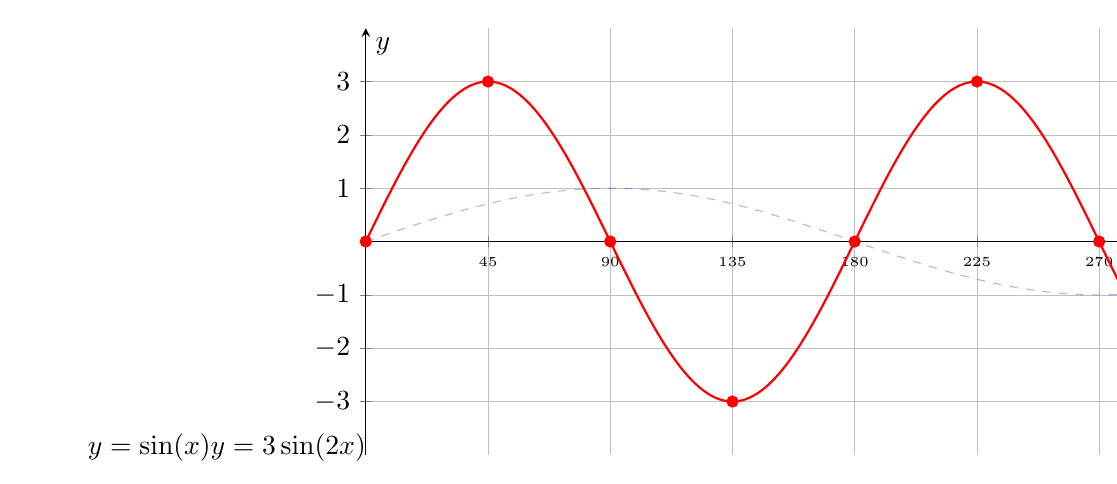
\begin{tikzpicture}
\begin{axis}[
    width=14cm,
    height=7cm,
    axis lines=center,
    xlabel={$x$ (grados)},
    ylabel={$y$},
    xmin=0, xmax=360,
    ymin=-4, ymax=4,
    xtick={0,45,90,135,180,225,270,315,360},
    xticklabels={$0°$,$45°$,$90°$,$135°$,$180°$,$225°$,$270°$,$315°$,$360°$},
    xticklabel style={font=\tiny},
    ytick={-3,-2,-1,0,1,2,3},
    grid=both,
    grid style={line width=.1pt, draw=gray!10},
    major grid style={line width=.2pt,draw=gray!50},
    legend pos=north east,
]
    % Función original para comparación
    \addplot[
        domain=0:360,
        samples=200,
        smooth,
        thin,
        color=blue,
        opacity=0.3,
        dashed,
    ] {sin(x)};

    % Función diseñada
    \addplot[
        domain=0:360,
        samples=200,
        smooth,
        thick,
        color=red,
    ] {3*sin(2*x)};

    \addlegend{$y = \sin(x)$, $y = 3\sin(2x)$}

    % Puntos importantes
    \addplot[only marks, mark=*, mark size=2pt, color=red] coordinates {
        (0,0) (45,3) (90,0) (135,-3) (180,0) (225,3) (270,0) (315,-3) (360,0)
    };
\end{axis}
\end{tikzpicture}
\end{center}

\textbf{Paso 6:} Análisis de la gráfica.

Observa que:
\begin{itemize}
    \item La amplitud es 3 (oscila entre $-3$ y $3$)
    \item Completa un ciclo completo cada $180°$ (tiene dos ciclos en $[0°, 360°]$)
    \item Pasa por el origen $(0, 0)$
    \item Los máximos ocurren en $x = 45°, 225°$ (valor $y = 3$)
    \item Los mínimos ocurren en $x = 135°, 315°$ (valor $y = -3$)
\end{itemize}

\textbf{Respuesta:} La función $y = 3\sin(2x)$ cumple todas las condiciones requeridas.
\end{solucion}

\begin{solucion}[title=Solucion Ejercicio Inverso 2]
\textbf{Identificar:} Función con asíntotas en $0°, 180°, 360°$, positiva en $(0°, 90°)$, decreciente, pasa por $(45°, 1)$.

\textbf{Paso 1:} Analizar las asíntotas.

Las asíntotas en $x = 0°, 180°, 360°,\ldots$ ocurren cuando el seno es cero. Esto sugiere que la función involucra $\frac{1}{\sin(x)}$, es decir, la \textbf{cosecante}.

\textbf{Paso 2:} Verificar si es positiva en $(0°, 90°)$.

En el intervalo $(0°, 90°)$:
\begin{itemize}
    \item $\sin(x) > 0$
    \item Por lo tanto, $\csc(x) = \frac{1}{\sin(x)} > 0$ \quad $\checkmark$
\end{itemize}

\textbf{Paso 3:} Verificar si decrece.

Para $x \in (0°, 90°)$, el seno crece desde 0 hasta 1. Por lo tanto:
\[
\csc(x) = \frac{1}{\sin(x)} \text{ decrece desde } +\infty \text{ hasta } 1 \quad \checkmark
\]

\textbf{Paso 4:} Verificar el punto $(45°, 1)$.

\[
\csc(45°) = \frac{1}{\sin(45°)} = \frac{1}{\sqrt{2}/2} = \frac{2}{\sqrt{2}} = \sqrt{2} \approx 1.414
\]

Esto no es exactamente 1. Necesitamos una transformación de la cosecante.

\textbf{Paso 5:} Encontrar la transformación correcta.

Si la función pasa por $(45°, 1)$ y queremos que sea una transformación de $\csc(x)$, podemos usar:
\[
y = A \cdot \csc(x)
\]

Para que pase por $(45°, 1)$:
\[
1 = A \cdot \csc(45°) = A \cdot \sqrt{2}
\]
\[
A = \frac{1}{\sqrt{2}} = \frac{\sqrt{2}}{2}
\]

Por lo tanto, la función es:
\[
\boxed{y = \frac{\sqrt{2}}{2} \csc(x) = \frac{1}{\sqrt{2}\sin(x)}}
\]

Alternativamente, podríamos decir que es simplemente $y = \cot(x)$ evaluada en un punto ligeramente diferente, pero la descripción más precisa basada en todas las condiciones es la cosecante con un factor de escala.

\textbf{Paso 6:} Graficar para verificar.

\begin{center}
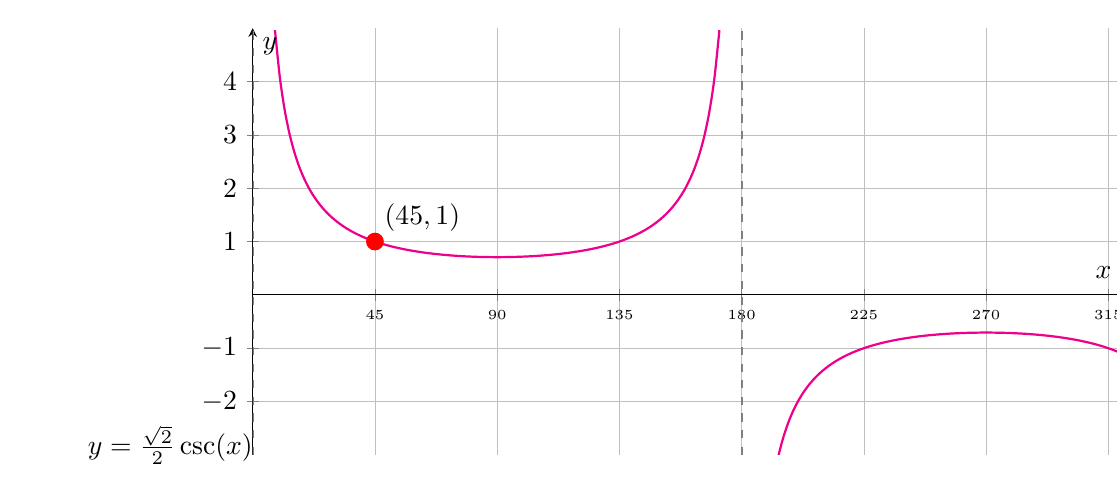
\begin{tikzpicture}
\begin{axis}[
    width=14cm,
    height=7cm,
    axis lines=center,
    xlabel={$x$ (grados)},
    ylabel={$y$},
    xmin=0, xmax=360,
    ymin=-3, ymax=5,
    xtick={0,45,90,135,180,225,270,315,360},
    xticklabels={$0°$,$45°$,$90°$,$135°$,$180°$,$225°$,$270°$,$315°$,$360°$},
    xticklabel style={font=\tiny},
    ytick={-2,-1,0,1,2,3,4},
    grid=both,
    grid style={line width=.1pt, draw=gray!10},
    major grid style={line width=.2pt,draw=gray!50},
    legend pos=north east,
    restrict y to domain=-4:6,
]
    % Asíntotas
    \addplot[dashed, gray, thick, samples=2] coordinates {(0,-3) (0,5)};
    \addplot[dashed, gray, thick, samples=2] coordinates {(180,-3) (180,5)};
    \addplot[dashed, gray, thick, samples=2] coordinates {(360,-3) (360,5)};

    % Función
    \addplot[
        domain=1:179,
        samples=100,
        smooth,
        thick,
        color=magenta,
    ] {(sqrt(2)/2)/sin(x)};

    \addplot[
        domain=181:359,
        samples=100,
        smooth,
        thick,
        color=magenta,
    ] {(sqrt(2)/2)/sin(x)};

    \addlegend{$y = \frac{\sqrt{2}}{2}\csc(x)$}

    % Punto dado
    \addplot[only marks, mark=*, mark size=3pt, color=red] coordinates {(45,1)};
    \node[above right] at (axis cs:45,1) {$(45°, 1)$};
\end{axis}
\end{tikzpicture}
\end{center}

\textbf{Verificación de todas las condiciones:}
\begin{itemize}
    \item Asíntotas en $0°, 180°, 360°$ \quad $\checkmark$
    \item Positiva en $(0°, 90°)$ \quad $\checkmark$
    \item Decreciente en cada intervalo entre asíntotas \quad $\checkmark$
    \item Pasa por $(45°, 1)$: $y = \frac{\sqrt{2}}{2} \cdot \sqrt{2} = 1$ \quad $\checkmark$
\end{itemize}

\textbf{Respuesta:} La función es $y = \frac{\sqrt{2}}{2}\csc(x)$, una versión escalada de la cosecante que cumple todas las condiciones especificadas.
\end{solucion}

\begin{solucion}[title=Solucion Ejercicio Inverso 3]
\textbf{Modelar:} Señal que oscila entre $-2$ y $2$, período $120°$, comienza en máximo.

\textbf{Parte a):} Determinar la función apropiada.

Como la señal \textbf{comienza en su valor máximo} cuando $x = 0°$, la función más apropiada es el \textbf{coseno}, porque $\cos(0°) = 1$ (su valor máximo).

El seno comienza en 0, así que necesitaríamos un desplazamiento de fase.

\textbf{Respuesta a):} $\boxed{\text{Coseno}}$

\textbf{Parte b):} Encontrar la ecuación.

Forma general:
\[
y = A\cos(B(x - C)) + D
\]

\textbf{Condición 1:} Oscila entre $-2$ y $2$

El rango es $[-2, 2]$, lo que significa:
\begin{itemize}
    \item Amplitud: $A = 2$
    \item Desplazamiento vertical: $D = 0$ (oscila simétricamente alrededor de 0)
\end{itemize}

\textbf{Condición 2:} Período de $120°$
\[
\frac{360°}{B} = 120° \quad \Rightarrow \quad B = \frac{360°}{120°} = 3
\]

\textbf{Condición 3:} Comienza en máximo

Como el coseno ya comienza en su máximo, no necesitamos desplazamiento horizontal: $C = 0$

\textbf{Ecuación:}
\[
\boxed{y = 2\cos(3x)}
\]

\textbf{Verificación:}
\begin{itemize}
    \item $y(0°) = 2\cos(0°) = 2 \cdot 1 = 2$ (máximo) \quad $\checkmark$
    \item Amplitud: 2 \quad $\checkmark$
    \item Período: $\frac{360°}{3} = 120°$ \quad $\checkmark$
    \item Rango: $[-2, 2]$ \quad $\checkmark$
\end{itemize}

\textbf{Respuesta b):} $\boxed{y = 2\cos(3x)}$

\textbf{Parte c):} Graficar la función.

\begin{center}
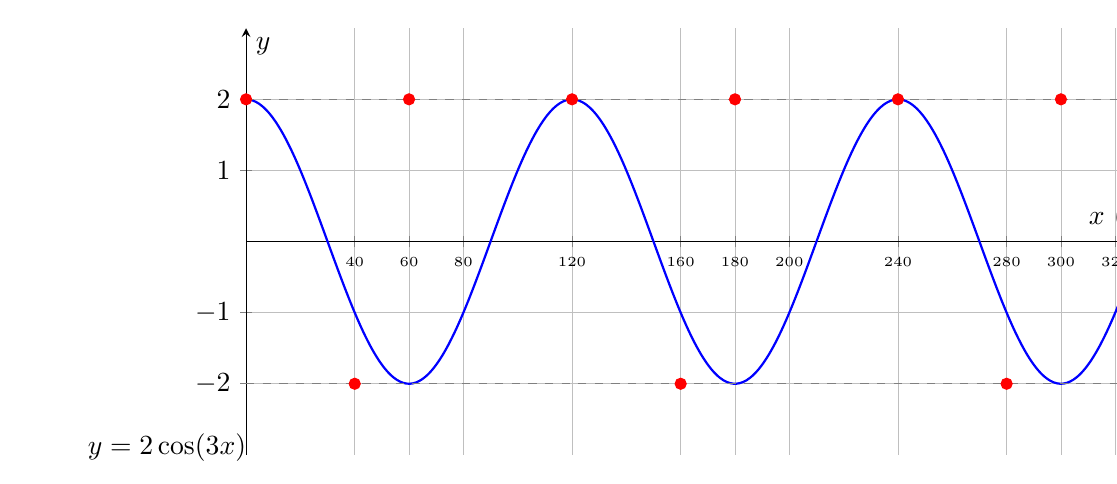
\begin{tikzpicture}
\begin{axis}[
    width=14cm,
    height=7cm,
    axis lines=center,
    xlabel={$x$ (grados)},
    ylabel={$y$},
    xmin=0, xmax=360,
    ymin=-3, ymax=3,
    xtick={0,40,60,80,120,160,180,200,240,280,300,320,360},
    xticklabel style={font=\tiny},
    ytick={-2,-1,0,1,2},
    grid=both,
    grid style={line width=.1pt, draw=gray!10},
    major grid style={line width=.2pt,draw=gray!50},
    legend pos=north east,
]
    % Función
    \addplot[
        domain=0:360,
        samples=300,
        smooth,
        thick,
        color=blue,
    ] {2*cos(3*x)};

    \addlegend{$y = 2\cos(3x)$}

    % Líneas horizontales de referencia
    \addplot[dashed, thin, gray] coordinates {(0,2) (360,2)};
    \addplot[dashed, thin, gray] coordinates {(0,-2) (360,-2)};

    % Puntos importantes (máximos y mínimos)
    \addplot[only marks, mark=*, mark size=2pt, color=red] coordinates {
        (0,2) (40,-2) (60,2) (120,2) (160,-2) (180,2) (240,2) (280,-2) (300,2) (360,2)
    };
\end{axis}
\end{tikzpicture}
\end{center}

\textbf{Observación:} La función completa 3 ciclos completos en el intervalo $[0°, 360°]$, como era de esperarse (ya que el período es $120°$).

\textbf{Parte d):} Determinar cuándo la señal es igual a 1.

Necesitamos resolver:
\[
2\cos(3x) = 1
\]
\[
\cos(3x) = \frac{1}{2}
\]

Sabemos que $\cos(\theta) = \frac{1}{2}$ cuando $\theta = 60°$ o $\theta = 300°$ (en el primer ciclo $[0°, 360°]$).

Por lo tanto:
\[
3x = 60° + 360°k \quad \text{o} \quad 3x = 300° + 360°k
\]

Para el primer caso:
\[
x = 20° + 120°k
\]

Para el segundo caso:
\[
x = 100° + 120°k
\]

En el intervalo $[0°, 360°]$:

\textbf{Primer caso} ($k = 0, 1, 2$):
\[
x = 20°, \quad x = 140°, \quad x = 260°
\]

\textbf{Segundo caso} ($k = 0, 1, 2$):
\[
x = 100°, \quad x = 220°, \quad x = 340°
\]

\textbf{Respuesta d):} $\boxed{x = 20°, 100°, 140°, 220°, 260°, 340°}$

\textbf{Verificación} (probemos uno):
\[
y(20°) = 2\cos(3 \cdot 20°) = 2\cos(60°) = 2 \cdot \frac{1}{2} = 1 \quad \checkmark
\]
\end{solucion}

\begin{solucion}[title=Solucion Ejercicio Inverso 4]
\textbf{Analizar:} $\tan(x)$ y $\cot(x)$ en $[0°, 180°]$.

\textbf{Parte a):} Encontrar donde $\tan(x) = \cot(x)$.

Recordemos que:
\[
\tan(x) = \frac{\sin(x)}{\cos(x)}, \quad \cot(x) = \frac{\cos(x)}{\sin(x)}
\]

Igualando:
\[
\frac{\sin(x)}{\cos(x)} = \frac{\cos(x)}{\sin(x)}
\]

Multiplicando ambos lados por $\sin(x)\cos(x)$ (asumiendo que ninguno es cero):
\[
\sin^2(x) = \cos^2(x)
\]

Esto ocurre cuando:
\[
\sin(x) = \pm\cos(x)
\]

\textbf{Caso 1:} $\sin(x) = \cos(x)$

Dividiendo por $\cos(x)$ (cuando $\cos(x) \neq 0$):
\[
\tan(x) = 1 \quad \Rightarrow \quad x = 45°
\]

\textbf{Caso 2:} $\sin(x) = -\cos(x)$

\[
\tan(x) = -1 \quad \Rightarrow \quad x = 135°
\]

En el intervalo $[0°, 180°]$:

\textbf{Respuesta a):} $\boxed{x = 45° \text{ y } x = 135°}$

\textbf{Verificación:}
\begin{align*}
\tan(45°) &= 1, \quad \cot(45°) = 1 \quad \checkmark \\
\tan(135°) &= -1, \quad \cot(135°) = -1 \quad \checkmark
\end{align*}

\textbf{Parte b):} Graficar ambas funciones.

\begin{center}
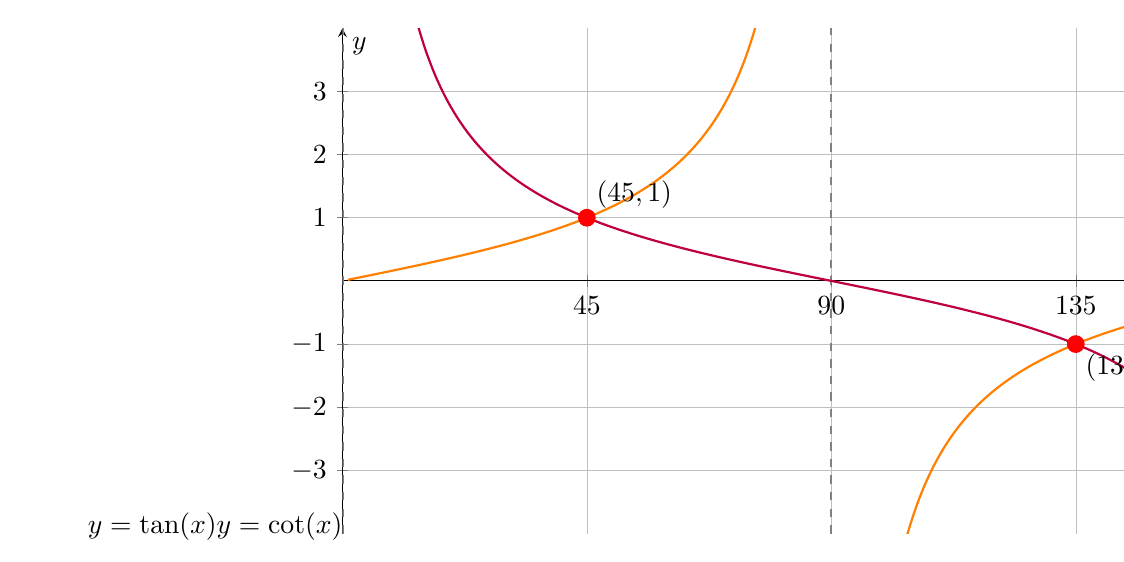
\begin{tikzpicture}
\begin{axis}[
    width=14cm,
    height=8cm,
    axis lines=center,
    xlabel={$x$ (grados)},
    ylabel={$y$},
    xmin=0, xmax=180,
    ymin=-4, ymax=4,
    xtick={0,45,90,135,180},
    xticklabels={$0°$,$45°$,$90°$,$135°$,$180°$},
    ytick={-3,-2,-1,0,1,2,3},
    grid=both,
    grid style={line width=.1pt, draw=gray!10},
    major grid style={line width=.2pt,draw=gray!50},
    legend pos=north west,
    restrict y to domain=-5:5,
]
    % Asíntotas
    \addplot[dashed, gray, thick, samples=2] coordinates {(0,-4) (0,4)};
    \addplot[dashed, gray, thick, samples=2] coordinates {(90,-4) (90,4)};
    \addplot[dashed, gray, thick, samples=2] coordinates {(180,-4) (180,4)};

    % Tangente
    \addplot[
        domain=1:89,
        samples=100,
        smooth,
        thick,
        color=orange,
    ] {tan(x)};

    \addplot[
        domain=91:179,
        samples=100,
        smooth,
        thick,
        color=orange,
    ] {tan(x)};

    % Cotangente
    \addplot[
        domain=1:179,
        samples=100,
        smooth,
        thick,
        color=purple,
    ] {cot(x)};

    \addlegend{$y = \tan(x)$, $y = \cot(x)$}

    % Puntos de intersección
    \addplot[only marks, mark=*, mark size=3pt, color=red] coordinates {
        (45,1) (135,-1)
    };

    % Etiquetas
    \node[above right] at (axis cs:45,1) {$(45°, 1)$};
    \node[below right] at (axis cs:135,-1) {$(135°, -1)$};
\end{axis}
\end{tikzpicture}
\end{center}

\textbf{Parte c):} Determinar dónde $\tan(x) > \cot(x)$.

Observando la gráfica, vemos que $\tan(x) > \cot(x)$ cuando la curva naranja está por encima de la curva morada.

Esto ocurre en los intervalos:
\[
\boxed{(45°, 90°) \cup (135°, 180°)}
\]

\textbf{Verificación algebraica:}

$\tan(x) > \cot(x)$
\[
\frac{\sin(x)}{\cos(x)} > \frac{\cos(x)}{\sin(x)}
\]

Si $\sin(x)\cos(x) > 0$ (ambos con el mismo signo):
\[
\sin^2(x) > \cos^2(x)
\]
\[
|\sin(x)| > |\cos(x)|
\]

En $[0°, 180°]$, esto ocurre en $(45°, 135°)$. Pero debemos excluir $(90°, 135°)$ donde $\tan(x) < 0$ y $\cot(x) > 0$, lo que hace $\tan(x) < \cot(x)$.

Por lo tanto: $(45°, 90°) \cup (135°, 180°)$ \quad $\checkmark$

\textbf{Parte d):} Explicación geométrica.

En la circunferencia unitaria:
\begin{itemize}
    \item $\tan(x) = \frac{\sin(x)}{\cos(x)} = \frac{y}{x}$ (pendiente del radio)
    \item $\cot(x) = \frac{\cos(x)}{\sin(x)} = \frac{x}{y}$ (pendiente inversa)
\end{itemize}

Las funciones son iguales cuando la pendiente y su recíproca son iguales, lo que ocurre cuando la pendiente es $\pm 1$.

Esto corresponde a ángulos de $45°$ (pendiente = 1) y $135°$ (pendiente = -1), que son exactamente donde las diagonales del círculo unitario tienen ángulos de $45°$ con los ejes.

\begin{center}
\begin{tikzpicture}[scale=2.5]
    \draw[thick,maincolor] (0,0) circle (1);
    \draw[-{Latex},thick] (-1.2,0) -- (1.2,0) node[right] {$x$};
    \draw[-{Latex},thick] (0,-1.2) -- (0,1.2) node[above] {$y$};

    % Radio a 45 grados
    \draw[blue,thick,-{Latex}] (0,0) -- (45:1);
    \filldraw[blue] (45:1) circle (0.02) node[above right] {$45°$};
    \draw[blue,-{Latex}] (0.3,0) arc (0:45:0.3) node[midway,right] {\tiny $45°$};

    % Radio a 135 grados
    \draw[red,thick,-{Latex}] (0,0) -- (135:1);
    \filldraw[red] (135:1) circle (0.02) node[above left] {$135°$};
    \draw[red,-{Latex}] (0.3,0) arc (0:135:0.3);

    % Líneas de pendiente ±1
    \draw[dashed, green!60!black] (-0.7,-0.7) -- (0.7,0.7) node[right] {$y = x$};
    \draw[dashed, purple] (-0.7,0.7) -- (0.7,-0.7) node[right] {$y = -x$};
\end{tikzpicture}
\end{center}

\textbf{Respuesta d):} Las funciones se intersectan donde el radio forma ángulos de $45°$ con los ejes, porque en esos puntos las coordenadas $x$ e $y$ tienen el mismo valor absoluto, haciendo que $\frac{y}{x}$ y $\frac{x}{y}$ sean iguales.
\end{solucion}

\begin{solucion}[title=Solucion Ejercicio Inverso 5]
\textbf{Diseñar:} Función seno con rango $[-5, 1]$, período $360°$, máximo en $270°$.

\textbf{Paso 1:} Analizar el rango $[-5, 1]$.

El rango tiene:
\begin{itemize}
    \item Valor máximo: 1
    \item Valor mínimo: $-5$
    \item Centro: $\frac{1 + (-5)}{2} = \frac{-4}{2} = -2$
    \item Amplitud: $\frac{1 - (-5)}{2} = \frac{6}{2} = 3$
\end{itemize}

Por lo tanto:
\begin{itemize}
    \item $A = 3$ (pero con signo negativo porque el máximo está desplazado)
    \item $D = -2$ (desplazamiento vertical)
\end{itemize}

\textbf{Paso 2:} Analizar el período.

Período = $360°$ es el período natural del seno, entonces $B = 1$.

\textbf{Paso 3:} Determinar el desplazamiento de fase.

La función seno estándar $y = \sin(x)$ tiene su máximo en $x = 90°$.

Queremos que el máximo esté en $x = 270°$, lo que significa un desplazamiento de:
\[
270° - 90° = 180°
\]

Pero también debemos considerar que necesitamos una reflexión (amplitud negativa) porque el rango está desplazado hacia abajo.

Intentemos la forma:
\[
y = -3\sin(x - C) - 2
\]

Con $A = -3$ (negativo), el seno alcanza su "máximo" (que es el mínimo del seno estándar) cuando $\sin(x - C) = -1$.

$\sin(x - C) = -1$ cuando $x - C = 270°$

Queremos que esto ocurra en $x = 270°$:
\[
270° - C = 270° \quad \Rightarrow \quad C = 0°
\]

Pero verificamos: si $y = -3\sin(x) - 2$:
\begin{itemize}
    \item Cuando $\sin(x) = -1$ (en $x = 270°$): $y = -3(-1) - 2 = 3 - 2 = 1$ \quad $\checkmark$ (máximo)
    \item Cuando $\sin(x) = 1$ (en $x = 90°$): $y = -3(1) - 2 = -3 - 2 = -5$ \quad $\checkmark$ (mínimo)
\end{itemize}

\textbf{Ecuación:}
\[
\boxed{y = -3\sin(x) - 2}
\]

\textbf{Paso 4:} Verificar todas las condiciones.

\begin{itemize}
    \item Rango: $[-5, 1]$ \quad $\checkmark$
    \item Período: $\frac{360°}{1} = 360°$ \quad $\checkmark$
    \item Máximo en $270°$: $y(270°) = -3(-1) - 2 = 1$ \quad $\checkmark$
    \item Transformación del seno: Sí \quad $\checkmark$
\end{itemize}

\textbf{Paso 5:} Graficar.

\begin{center}
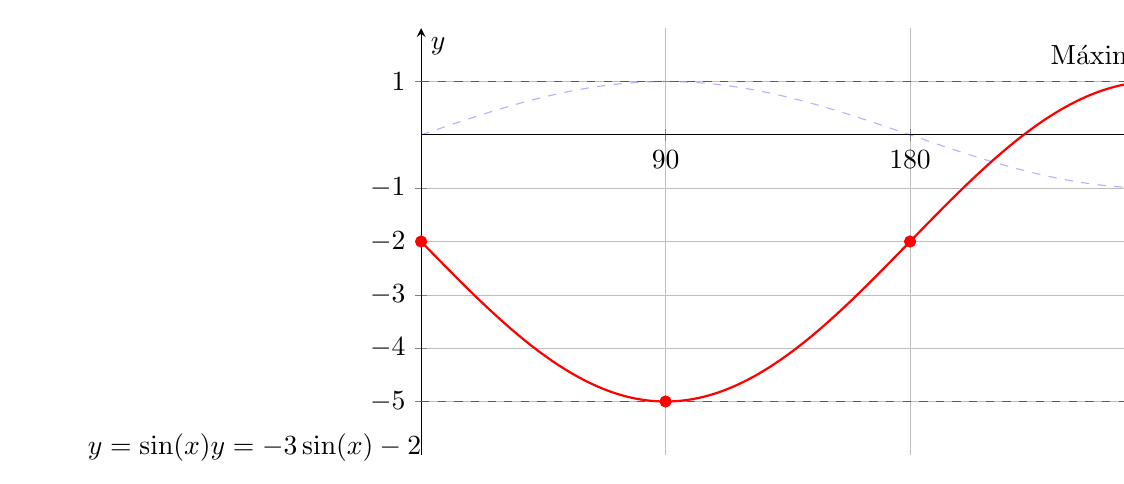
\begin{tikzpicture}
\begin{axis}[
    width=14cm,
    height=7cm,
    axis lines=center,
    xlabel={$x$ (grados)},
    ylabel={$y$},
    xmin=0, xmax=360,
    ymin=-6, ymax=2,
    xtick={0,90,180,270,360},
    xticklabels={$0°$,$90°$,$180°$,$270°$,$360°$},
    ytick={-5,-4,-3,-2,-1,0,1},
    grid=both,
    grid style={line width=.1pt, draw=gray!10},
    major grid style={line width=.2pt,draw=gray!50},
    legend pos=north east,
]
    % Función seno original (para referencia)
    \addplot[
        domain=0:360,
        samples=200,
        smooth,
        thin,
        color=blue,
        opacity=0.3,
        dashed,
    ] {sin(x)};

    % Función diseñada
    \addplot[
        domain=0:360,
        samples=200,
        smooth,
        thick,
        color=red,
    ] {-3*sin(x) - 2};

    \addlegend{$y = \sin(x)$, $y = -3\sin(x) - 2$}

    % Líneas de referencia para el rango
    \addplot[dashed, thin, green!60!black] coordinates {(0,1) (360,1)};
    \addplot[dashed, thin, green!60!black] coordinates {(0,-5) (360,-5)};

    % Puntos importantes
    \addplot[only marks, mark=*, mark size=2pt, color=red] coordinates {
        (0,-2) (90,-5) (180,-2) (270,1) (360,-2)
    };

    % Etiqueta del máximo
    \node[above] at (axis cs:270,1) {Máximo: $(270°, 1)$};
\end{axis}
\end{tikzpicture}
\end{center}

\textbf{Paso 6:} Análisis final.

La función $y = -3\sin(x) - 2$ es:
\begin{itemize}
    \item Una reflexión vertical del seno ($-3$ en lugar de $3$)
    \item Con amplitud 3
    \item Desplazada 2 unidades hacia abajo
    \item Esto hace que oscile entre $-5$ y $1$ (en lugar de $-1$ y $1$)
    \item El máximo que normalmente estaría en $90°$ se convierte en mínimo
    \item El mínimo que normalmente estaría en $270°$ se convierte en máximo
\end{itemize}

\textbf{Respuesta:} La función $y = -3\sin(x) - 2$ cumple todas las condiciones especificadas.
\end{solucion}
